\subsection{拓扑与初始资金配置的四臂补充分析}

为区分搜索后拓扑差异与初始资金配置差异，在已有父图上开展事后四臂分析。将需求感知构造记为DA，分别固定DA和FHS5拓扑；U表示按节点参与坐标作商余数均匀分配，O表示原共同资金优化产生的初态。四臂为DA-U、FHS5-U、DA-O和FHS5-O，每节点预算均为120。两条O臂复用原受核验结果，U臂使用同一留出请求及请求级路由票据。改变配置可改变超边资金总额，故这里控制的是节点预算，而非固定每条超边资金的纯拓扑因果干预。

对第2节定义的两个终点分别计算
\begin{equation}
\begin{aligned}
\Delta_U&=\overline Z_{\mathrm{DA-U}}-\overline Z_{\mathrm{FHS5-U}},\\
\Delta_O&=\overline Z_{\mathrm{DA-O}}-\overline Z_{\mathrm{FHS5-O}},\\
\Gamma&=\Delta_O-\Delta_U,
\end{aligned}\label{eq:s5-interaction}
\end{equation}
其中$Z$取归一化受限无路径时间或窗口内失败指示。$\Gamma$也等于两拓扑各自O减U之差，因此直接反映拓扑对比随初始化变化的幅度。交互由共享重抽样逐次直接计算，不以一项区间含零、另一项不含零判断差异。

每相位、每规模仍有60个独立父图，3个模型各20个；7条轨迹先在父图内等权平均，再对模型均值等权汇总。在Python 3.12.14中，每相位、每规模进行20\,000次模型分层整父图配对重抽样，四臂和两个终点共用索引，采用第500和19\,500顺序统计量形成点态95\% percentile区间。全部80项合并范围比较均报告，未作多重比较校正；同分布和分布偏移的160项对比仅作描述。相位标签沿用原数据，这项事后分析不是新的预注册或盲确认实验，也不沿用主分析的家族复现判据。

均匀初态下，30节点DA相对FHS5的归一化时间差在正式和确认相位分别为0.002077和0.001171；60节点分别为0.000003和$-0.000017$。240节点两相位的经验拓扑差均为0。完整拓扑差和交互见补充图S2，不能据零宽经验区间断言总体等效。图\ref{fig:s5-initialization}进一步展示各拓扑内部的O减U：16个相位、规模和拓扑条件中，归一化时间差点估计15个为负、1个为正；这只是条件方向计数，不是16个独立重复或统计检验。确认相位240节点两拓扑的时间差均为$-0.005575$，点态区间为$[-0.012888,-0.000705]$；失败风险均增加1.667个百分点，点态区间为$[0.238,3.571]$个百分点。

\begin{figure*}[t]\centering
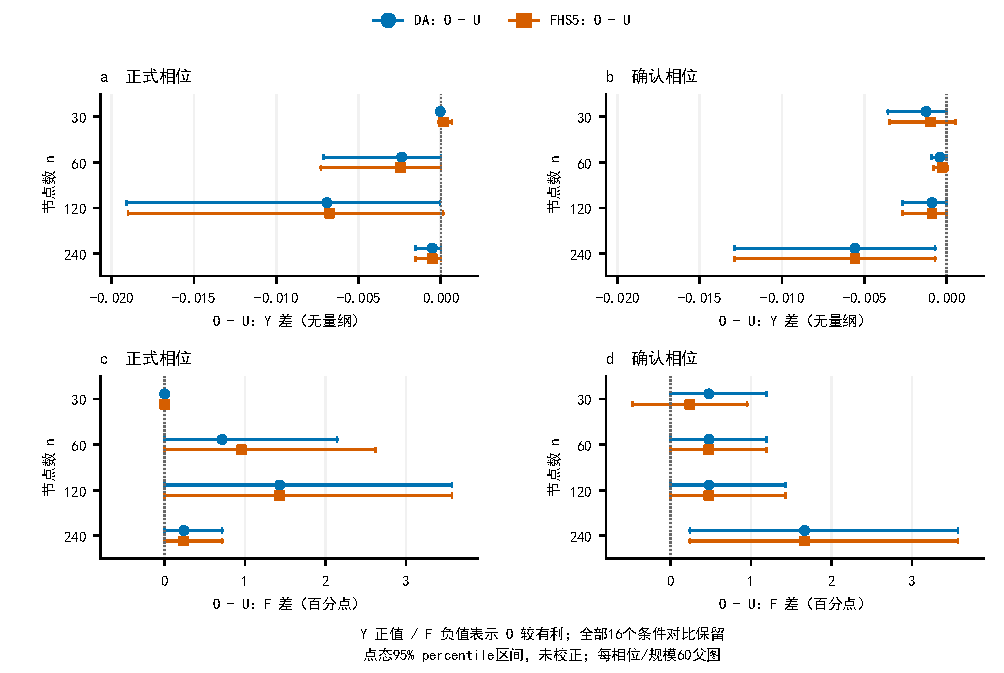
\includegraphics[width=170mm]{figures/s5-initialization.pdf}
\caption{固定拓扑内的初态对比。a、b为正式、确认相位的归一化受限时间差；c、d为对应失败风险差（百分点）。圆点与方块分别为DA和FHS5的O减U估计，横线为点态、未校正95\%区间；每相位、每规模60父图，模型各20，7条轨迹先在父图内汇总。时间差正值、风险差负值表示O较有利；无显著性星号。全部条件保留，源数据见补充材料。}\label{fig:s5-initialization}
\end{figure*}

这些观察不支持原优化初态普遍优于均匀初态，也不证明所有资金优化有害。结构搜索依据训练需求的静态代理目标，资金配置则依据有限训练情景的受限时间字典序评分；二者均不保证留出服务终点改善。当前四臂数据揭示了训练选择与留出表现的差距，但未识别其机制。主分析中超图相对二元参照的资源匹配收益，与DA相对FHS5的搜索增量、O相对U的配置增量，是不同估计对象，不能相互替代。
